\chapter{Géometrie vectorielle}


Dans ce chapitre, nous allons utiliser certaines notions de l'algèbre linéaire pour
étudier la géométrie vectorielle dans $\BBR^3$, également connu sous le nom
d'\definition{espace euclidien à trois dimensions}.   
Nous allons nous intéresser à quatre type d'objets: 1) les points, objet à
zéro dimension, que nous
allons représenter par 2) des vecteurs; 3) les droites, qui sont des objets
ayant une dimension, et 4) les plans, qui sont des objets à deux dimensions.

Avant de débuter la matière du chapitre, répondez à la question suivante.

\begin{exerciceC}
Vrai ou faux: l'équation $y=mx+b$ représente une droite.
\end{exerciceC}

\section{Notation utilisée dans ce chapitre}
Dans ce chapitre, nous allons utiliser une notation légèrement différente de celle
utilisée dans le reste de ce livre pour adopter une notation traditionnellement utilisée
dans les cours d'introduction aux vecteurs dans l'espace euclidien ($\BBR^3$) ainsi
que dans les sciences naturelles telle que la physique.  Ainsi, un vecteur sera
représenté soit par un symbole surmonté d'une flèche, $\vect{r}$, ou
par un triplet de nombres, $(x, y, z)$ qui est simplement un 
vecteur ligne\footnote{C'est-à-dire une matrice $1\times 3$} où
on utilise des virgules pour séparer les coefficients dans le but d'éviter toute
ambiguïté. Nous allons utiliser la base de vecteurs suivante:
\[
\begin{matrix}[rcl]
\iunit &=& (1, 0, 0) \qquad \explain{vecteur unitaire le long de l'axe des $x$}\\
\junit &=& (0, 1, 0) \qquad \explain{vecteur unitaire le long de l'axe des $y$}\\
\kunit &=& (0, 0, 1) \qquad \explain{vecteur unitaire le long de l'axe des $z$}
\end{matrix}
\]
ce qui nous donne une autre façon de représenter un vecteur:
\[
\vect{r} = (x, y, z) = x\iunit + y\junit + z\kunit
\]
Avec la notation que nous avons utilisée dans les autres chapitres, avec $\{\mat{e}_j\}$ comme
base de l'espace vectoriel, nous aurions plutôt écrit:
\[
\mat{r} = \begin{pmatrix}
x \\ y \\ z
\end{pmatrix} = x\mat{e}_1 + y\mat{e}_2 + z\mat{e}_3
\]

\section{Produit scalaire}
Nous avons déjà vu le produit scalaire de deux vecteurs, 
$\langle \mat{u}, \mat{v}\rangle = \tr(\transp{\mat{v}}, \mat{u})$.  
Dans la notation utilisée dans ce chapitre, nous écrivons le produit scalaire de la façon suivante:
\[
\vect{u}\cdot\vect{v} = u_1 v_1 + u_2 v_2 + u_3 v_3
\]
Supposons que nous choisissons l'orientation de notre système d'axes de telle sorte 
que le vecteur $\vect{u}$ est dans le plan $xy$ et que le vecteur 
$\vect{v}$ est le long de l'axe des $x$ tel
qu'illustré à la figure \ref{fig:dot-prod}.
\[
\begin{matrix}[rcl]
\vect{u} &=& (a, b, 0) \\
\vect{v} &=& (v, 0, 0)
\end{matrix}
\]
Si on fait le calcul, on trouve que le produit scalaire est $\vect{u}\cdot\vect{v} = av$.  
En examinant la figure  \ref{fig:dot-prod}, on constate que $a = u\cos\theta$ de telle sorte
que\footnote{Ce résultat est ce que nous avions défini à l'équation \eqref{eq:cos} pour
le cosinus de l'angle entre deux vecteurs.} $\vect{u}\cdot\vect{v} = uv\cos\theta$ 
où $u=\norm{\vect{u}}$ et $v=\norm{\vect{v}}$.

\begin{figure}[h]
\begin{center}
\begin{tikzpicture}
	\coordinate (A0) at (0, 0);
	\coordinate (B0) at (1, 2);
	\coordinate (C0) at (3, 0);
	\coordinate (D0) at (3.5, 1);
% initial area
%\path [fill=blue!10] (A0) -- (B0) -- (D0) -- (C0) -- (A0);
	% les axes
	\draw[->,thin,black!70] (-0.5,0) -- (3.5,0) node[anchor=west]{x};
	\draw[->,thin,black!70] (0,-0.5) -- (0,3) node[anchor=south]{y};
	% les deux vecteurs
	\draw[->,thick,blue] (A0) node[anchor=south west]{\color{black}$\quad\theta$} --  node[anchor=east]{$\vect{u}$} (B0);
	\draw[->,thick,blue] (A0) --  node[anchor=north]{$\vect{v}$} (C0);
	\draw [black] (0.5,0) arc [radius=0.5, start angle=0, end angle= 60];
	% tick marks
	\draw[-,thin,black!70] (-0.1, 2) node[anchor=east]{\tiny b} -- (0.1,2);
	\draw[-,thin,black!70] (1, -0.1) node[anchor=north]{\tiny a} -- (1, 0.1);
	\draw[-,thin,black!70] (3, -0.1) node[anchor=north]{\tiny $v$} -- (3, 0.1);
	\draw[dotted, blue] (1, 0) -- (B0);
\end{tikzpicture}
\caption{ \label{fig:dot-prod}Deux vecteurs séparés par un angle $\theta$. Lorsqu'on fait le produit scalaire de ces deux
vecteurs, ceci revient à multiplier la longueur d'un de ces deux vecteurs $(v = \norm{\vect{v}})$ par la projection de l'autre $(u\cos\theta = a)$.
}
\end{center}
\end{figure}

\section{Produit vectoriel}
Soient les vecteurs $\vect{u}, \vect{v}, \vect{w} \in\BBR^3$.  Nous pouvons construire une matrice $3\times 3$ telle que chaque ligne est un de ces vecteurs:
\[
\matM = \begin{pmatrix}
\vect{u}\\
\vect{v}\\
 \vect{w}
\end{pmatrix}
= \begin{pmatrix}
u_1 & u_2 & u_3 \\
v_1 & v_2 & v_3 \\
w_1 & w_2 & w_3 
\end{pmatrix}
\]
Si on calcule le déterminant de cette matrice\footnote{Puisque le déterminant d'une matrice
et de sa transposée sont égaux, on aurait pu définir une telle matrice en utilisant chaque
vecteur comme une colonne de la matrice plutôt que comme une ligne.}
 en faisant l'expansion par la première rangée, on trouve:
\[
|\matM| = \begin{vmatrix}
u_1 & u_2 & u_3 \\
v_1 & v_2 & v_3 \\
w_1 & w_2 & w_3
\end{vmatrix}
= u_1 \begin{vmatrix}
v_2 & v_3 \\
w_2 & w_3
\end{vmatrix}
-
u_2 \begin{vmatrix}
v_1 & v_3 \\
w_1 & w_3
\end{vmatrix}
+
u_3 \begin{vmatrix}
v_1 & v_2 \\
w_1 & w_2
\end{vmatrix}
\]
On peut écrire ceci comme un produit scalaire de deux vecteurs:
\[
|\matM| =(u_1\iunit + u_2\junit+u_3\kunit) \cdot
\left( \begin{vmatrix}
v_2 & v_3 \\
w_2 & w_3
\end{vmatrix} \iunit
-
\begin{vmatrix}
v_1 & v_3 \\
w_1 & w_3
\end{vmatrix}\junit
+
 \begin{vmatrix}
v_1 & v_2 \\
w_1 & w_2
\end{vmatrix}\kunit\right)
\]
Nous définissons le \definition{produit vectoriel} des vecteurs $\vect{v}, \vect{w}$ comme étant
le deuxième vecteur apparaissant dans le produit scalaire ci-dessus:
\[
\vect{v}\times \vect{w} =
 \begin{vmatrix}
v_2 & v_3 \\
w_2 & w_3
\end{vmatrix} \iunit
- \begin{vmatrix}
v_1 & v_3 \\
w_1 & w_3
\end{vmatrix}\junit
+
 \begin{vmatrix}
v_1 & v_2 \\
w_1 & w_2
\end{vmatrix}\kunit =
  \begin{vmatrix}[ccc]
\iunit &\junit &\kunit \\
 v_1 & v_2 & v_3 \\
 w_1 & w_2 & w_3
 \end{vmatrix}
\]
de telle sorte que, avec cette définition, le déterminant de la matrice $\matM$ peut être écrit:
\[
 \begin{vmatrix}
\vect{u}\\
\vect{v}\\
 \vect{w}
\end{vmatrix} = \vect{u}\cdot (\vect{v} \times \vect{w})
\]
l'expression $\vect{u}\cdot (\vect{v} \times \vect{w})$ étant connue sous le nom de \definition{produit mixte}.
Quelques remarques sur le produit vectoriel:
\begin{enumerate}
\item Puisque le déterminant d'une matrice qui a deux lignes identiques est égal à zéro, cela veut
dire que si on choisit $\vect{u} = \vect{v}$, le déterminant sera nul, et donc 
$\vect{v} \cdot (\vect{v}\times\vect{w}) = 0$
ce qui veut dire que le vecteur $\vect{v}\times\vect{w}$ est orthogonal au vecteur $\vect{v}$.
\item De la même façon, si on choisit $\vect{u} = \vect{w}$, on conclut que 
 le vecteur $\vect{v}\times\vect{w}$ est orthogonal au vecteur $\vect{w}$.
 \item Le vecteur  $\vect{v}\times\vect{w}$ est donc perpendiculaire au plan engendré par les
 vecteurs  $\vect{v}$ et  $\vect{w}$.

 \item Puisque le déterminant change de signe si on interchange deux lignes, on en conclut que
 \[
 \vect{v}\times\vect{w} = - \vect{w}\times\vect{v}
 \]
 \item On observe que le produit vectoriel d'un vecteur par lui-même est nul: $\vect{v}\times\vect{v}=\vect{0}$
 \item La direction d'un vecteur résultant d'un produit vectoriel est donné par la \textit{règle de la main droite} illustrée par
 la figure dans la marge.
 %
 \begin{marginfigure}
 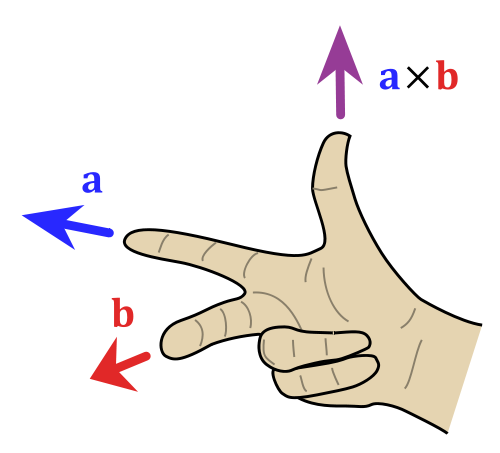
\includegraphics[width=1.8in]{images/main-droite.png}
 \caption{Règle de la main droite donnant la direction d'un produit vectoriel.}\label{image:main-droite}
 \end{marginfigure}
 %
 \item Le résultat d'un produit vectoriel est un \textit{pseudo-vecteur}: si fait une réflexion par rapport aux
 trois axes, un vecteur change de signe alors qu'un pseudo-vecteur reste inchangé.
 \item Le produit vectoriel n'est pas une opération définie dans tous les espaces vectoriels: on peut
 seulement le définir\footnote{La preuve pour ceci requiert des notions
  allant au-delà de ce cours.}
   dans $\BBR^3$ et $\BBR^7$; 
   dans ce dernier cas, le produit ne peut pas être exprimé comme un simple déterminant
 de la même façon que nous avons défini le produit vectoriel dans $\BBR^3$.
 \end{enumerate}
 
\noindent Finalement, calculons la longueur de ce vecteur:
 \[ 
 \begin{matrix}[rcl]
\norm{\vect{v}\times\vect{w}}^2 &=& (v_2 w_3 - v_3 w_2)^2 + (v_1 w_3 - v_3 w_1)^2 + (v_1 w_2 - v_2 w_1)^2 \\
&=& (v_2 w_3)^2 + (v_3 w_2)^2 - 2(v_2 v_3 w_2 w_3) + (v_1 w_3)^2 + (v_3 w_1)^2 - 2 (v_1 v_3 w_1 w_3) \\
 && +\, (v_1 w_2)^2 + (v_2 w_1)^2  -2(v_1 v_2 w_1 w_2) \\
 &&  \qquad {\color{blue} +\, (v_1 w_1)^2 + (v_2w_2)^2 + (v_3 w_3)^2} \\
  &&  \qquad {\color{red} -\, (v_1 w_1)^2 - (v_2w_2)^2 - (v_3 w_3)^2} \\
  &=& v_1^2(w_1^2 + w_2^2 + w_3^2) + v_2^2(w_1^2+w_2^2+w_3^2)  + v_3^2(w_1^2+w_2^2+w_3^2) \\
  &&  -\, (v_1 w_1)^2 - (v_2w_2)^2 - (v_3 w_3)^2 -2(v_1 v_2 w_1 w_2) - 2 (v_1 v_3 w_1 w_3) - 2(v_2 v_3 w_2 w_3) \\
  &=& (v_1^2 + v_2^2 + v_3^2)(w_1^2 + w_2^2 + w_3^2) - (u_1v_1 + u_2v_2 + u_3 v_3)^2 \\
  &=& \norm{\vect{v}}^2 \norm{\vect{w}}^2 - (\vect{v}\cdot\vect{w})^2 \\
  &=&  \norm{\vect{v}}^2 \norm{\vect{w}}^2 -  \norm{\vect{v}}^2 \norm{\vect{w}}^2\cos^2\theta \\
  &=&  \norm{\vect{v}}^2 \norm{\vect{w}}^2 (1-\cos^2\theta) \\
  &=&  \norm{\vect{v}}^2 \norm{\vect{w}}^2 \sin^2\theta
 \end{matrix}
 \]
 
\noindent On obtient donc 
$\norm{\vect{v}\times\vect{w}} =  \norm{\vect{v}} \norm{\vect{w}} \sin\theta = vw\sin\theta$ 
où $\theta$ est l'angle entre les deux vecteurs.

\begin{exemple}\label{exemple-prod-vect}
Soient les vecteurs $\vect{v} = (1, 2, 3)$ et $\vect{u} = (0, 4, -5)$.
\partexemple{a} Calculez le produit scalaire $\vect{v}\cdot\vect{u}$.
\partexemple{b} Calculez le produit vectoriel $\vect{v}\times \vect{u}$.
\solution
\partexemple{a} Le produit  scalaire 
\[
\begin{matrix}[rcl]
\vect{v}\cdot\vect{u} &=& (1, 2, 3) \cdot (0, 4, -5) \\
 &=& 1\cdot 0 + 2\cdot 4 + 3\cdot (-5) = -7 
\end{matrix}
\]
On note que ces vecteurs ne sont pas orthogonaux parce que leur produit
scalaire n'est pas nul.
\partexemple{b} Le produit vectoriel $\vect{v}\times \vect{u}$ est obtenu
en calculant le déterminant suivant:
\[
\vect{v}\times \vect{u} = \begin{vmatrix}
\iunit & \junit & \kunit \\
1 & 2 & 3 \\
0 & 4 & -5
\end{vmatrix}
\] 
Pour calculer un tel déterminant, il est toujours plus simple de faire l'expansion
par la première ligne car ceci nous donne directement les composantes du nouveau vecteur.
Nous avons donc
\[
\begin{matrix}[rcl]
\vect{v}\times \vect{u}= \begin{vmatrix}
\iunit & \junit & \kunit \\
1 & 2 & 3 \\
0 & 4 & -5
\end{vmatrix} &=& \iunit \begin{vmatrix}
2 & 3 \\ 4 & -5
\end{vmatrix}\
-\junit \begin{vmatrix}
1 & 3 \\ 0 & -5
\end{vmatrix} 
+ \kunit \begin{vmatrix}
1 & 2 \\ 0 & 4
\end{vmatrix} \\
&=& -22 \iunit + 5 \junit + 4\kunit
\end{matrix}
\] 
et donc 
$\vect{v}\times \vect{u} = (-22, 5, 4)$.  
On note que ces vecteurs ne sont pas parallèles parce que leur produit vectoriel
n'est pas nul.
\end{exemple}

\begin{exerciceC}\label{ex:prop-vect}
Vérifiez que les propriétés suivantes des vecteurs unitaires sont satisfaites.
\[
\begin{cases}
\iunit\times\junit=\kunit = -\junit\times\iunit\\
\junit\times\kunit=\iunit = -\kunit\times\junit\\
\kunit\times\iunit=\junit = -\iunit\times\kunit\\
\iunit\times\iunit=\junit\times\junit=\kunit\times\kunit=0\end{cases}\]
\suggestion{$\iunit = (1, 0, 0)$}
\end{exerciceC}

Les vecteurs de l'exemple précédent ne sont ni orthogonaux, ni parallèles.  
On peut calculer de deux façons l'angle entre ces deux vecteurs, tel qu'illustré
dans l'exemple suivant.

\begin{exemple}
Calculez l'angle entre les vecteurs $\vect{v} = (1, 2, 3)$ et $\vect{u} = (0, 4, -5)$.

\solution
Comme nous avons déjà calculé le produit scalaire ainsi que le produit vectoriel
de ces deux vecteurs dans l'exemple précédent, à première vue on pourrait penser
qu'on pourrait soit utiliser
$\vect{v}\cdot\vect{u} = uv\cos\theta$ ou $\norm{\vect{v}\times\vect{u}} = uv\sin\theta$
pour déterminer l'angle $\theta$ entre ces deux vecteurs.  Dans les deux cas, nous
devons calculer la norme de chacun de ces vecteurs.  Nous avons
\[
v = \norm{\vect{v}} = \sqrt{\vect{v}\cdot\vect{v}} = \sqrt{1^2 + 2^2 + 3^2} = \sqrt{14}
\]
et
\[
u = \norm{\vect{u}} = \sqrt{\vect{u}\cdot\vect{u}} = \sqrt{0^2 + 4^2 + (-5)^2} = \sqrt{41}
\]
Comme nous avons trouvé que $\vect{v}\cdot\vect{u}=-7$, nous obtenons
\[
\cos\theta = \frac{-7}{\sqrt{14}\sqrt{41}} \Rightarrow \theta = 1,867\ldots \mbox{rad ou approx. $107$ degrés}
\]
Nous aurions pu également utiliser le résultat du produit vectoriel.
\[
\norm{\vect{v}\times\vect{u}} = \sqrt{(-22, 5, 4)\cdot(-22, 5, 4)} = \sqrt{525}
\]
et
\[
\sin\theta = \frac{\sqrt{525}}{\sqrt{14}\sqrt{41}} = 73,01\ldots\mbox{degrés} \ldots\quad\mbox{ou }107 \quad [=180-73]
\]
Comme on le voit, si on utilise le produit vectoriel, on ne peut pas décider si l'angle est entre 0 et $\pi/2$ ou
entre $\pi/2$ et $\pi$, tel qu'illustré à la figure \ref{fig:cross-prod}; 
pour cette raison, il est préférable d'utiliser le produit scalaire pour déterminer l'angle entre les vecteurs.
\end{exemple}


Habituellement, lorsque le produit vectoriel est présenté pour la première fois,
la méthode de calcul choisie utilise les propriétés du produit vectoriel des vecteurs unitaires
telle que listée à l'\refexercice{ex:prop-vect}
et présente la multiplication suivant le même modèle qu'on utiliserais pour
multiplier des polynômes, plutôt que d'utiliser l'expansion d'un déterminant.
L'exemple suivant démontre ceci.
\begin{exemple}
Calculez le produit vectoriel des vecteurs $\vect{v} = (1, 2, 3)$ et $\vect{u} = (0, 4, -5)$.
\solution
Comme nous pouvons écrire $\vect{v} = \iunit + 2\junit + 3 \kunit$ et 
$\vect{u} = 4\junit - 5\kunit$, nous avons
\[
\begin{matrix}[rcl]
\vect{v}\times\vect{u} &=& (\iunit + 2\junit + 3 \kunit)\times(4\junit - 5\kunit) \\
&=& 4\iunit\times\junit -5\iunit\times\kunit + 2\cdot4\junit\times\junit -2\cdot5\junit\times\kunit + 3\cdot4\kunit\times\junit -3\cdot5\kunit\times\kunit\\
&=& 4\kunit +5\junit + 0 -10\iunit -12\iunit + 0\\
&=& -22\iunit + 5\junit +4\kunit
\end{matrix}
\]
et donc, $\vect{v}\times \vect{u} = (-22, 5, 4)$ comme on l'avait vu à
l'\refexemple{exemple-prod-vect}.
\end{exemple}


\begin{exerciceC}
Calculez le produit scalaire, le produit vectoriel et l'angle entre les vecteurs
$\vect{u} = (3, -5, 4)$ et $\vect{v} = (3, 5, 4)$.  Utilisez la méthode du déterminant
pour calculer le produit vectoriel.
\end{exerciceC}
\begin{exerciceC}
Calculez le produit scalaire, le produit vectoriel et l'angle entre les vecteurs
$\vect{u} = (3, -5, 4)$ et $\vect{v} = (2, -1, 0)$.  Utilisez la méthode du produit
de polynômes pour calculer le produit vectoriel.
\end{exerciceC}

\subsection{Interprétation géométrique de la norme du produit vectoriel}

Supposons que nous avons deux vecteurs, $\vect{u}$ et $\vect{v}$ et que nous
choisissions\footnote{Peu importe les deux vecteurs qu'on nous donne,
il est toujours possible de choisir un système d'axes ayant l'orientation
que nous décrivons.} nos axes de telle sorte que $\vect{u}$ soit orienté le long de l'axe
des $x$, $\vect{u} = (u, 0, 0)$, et que $\vect{u}$ soit dans le plan $xy$, 
$\vect{v} = (a, b, 0)$, tel qu'illustré sur la figure \ref{fig:cross-prod}.
Le produit vectoriel $\vect{u}\times\vect{v}$ est obtenu en
calculant le déterminant:
\[
\vect{u}\times\vect{v} = 
\begin{vmatrix}
\iunit & \junit & \kunit\\
u & 0 & 0 \\
a & b & 0 
\end{vmatrix}
\]
Puisque la troisième colonne ne contient qu'un terme non-nul, le calcul
du déterminant est simplifié si on fait l'expansion suivant cette colonne:
\[
\vect{u}\times\vect{v} = \kunit
\begin{vmatrix}
u & 0 \\
a & b
\end{vmatrix} = ub\, \kunit
\]
Ceci nous donne une interprétation géométrique\footnote{Puisqu'on a choisi de définir le produit
vectoriel en partant d'un déterminant d'une matrice de trois vecteurs, 
nous avions essentiellement déjà vu ceci dans la section \ref{sec:det-geom}.
Dans la plupart des autres livres, on présente une autre définition du produit vectoriel
et le calcul en utilisant un déterminant est présenté comme un "truc" utile.}: 
la norme de ce produit est $ub$ ce qui est égal à l'aire du parallélogramme engendré par les 
deux vecteurs $\vect{u}$ et $\vect{v}$. 
En examinant la figure  \ref{fig:cross-prod}, on observe que
$b=v\sin\theta$ et donc on peut écrire la norme comme étant $uv\sin\theta$ comme
on l'avait obtenu auparavant dans le cas général.
\begin{figure}[h]
\begin{center}
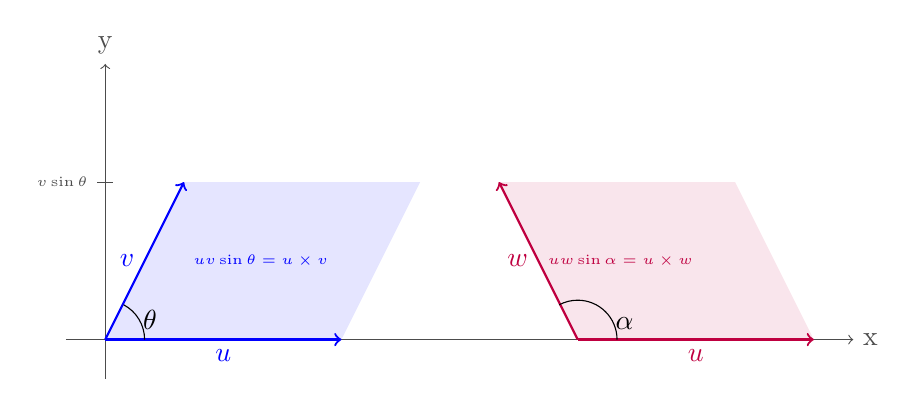
\begin{tikzpicture}
	\coordinate (A0) at (0, 0);
	\coordinate (B0) at (1, 2);
	\coordinate (C0) at (3, 0);
	\coordinate (D0) at (4, 2);
	%
	\coordinate (A1) at (6, 0);
	\coordinate (B1) at (5, 2);
	\coordinate (C1) at (9, 0);
	\coordinate (D1) at (8, 2);	
	
	
% initial area
\path [fill=blue!10] (A0) -- (B0) -- (D0) -- (C0) -- (A0);
\path [fill=purple!10] (A1) -- (B1) -- (D1) -- (C1) -- (A1);
	% les axes
	\draw[->,thin,black!70] (-0.5,0) -- (9.5,0) node[anchor=west]{x};
	\draw[->,thin,black!70] (0,-0.5) -- (0,3.5) node[anchor=south]{y};
	% les vecteurs
	\draw[->,thick,blue] (A0) node[anchor=south west]{\color{black}$\quad\theta$} --  node[anchor=east]{$\vect{v}$} (B0);
	\draw[->,thick,blue] (A0) --  node[anchor=north]{$\vect{u}$} (C0);
	\draw [black] (0.5,0) arc [radius=0.5, start angle=0, end angle= 62];
	%
	% les vecteurs
	\draw[->,thick,purple] (A1) node[anchor=south west]{\color{black}$\quad\alpha$} --  node[anchor=east]{$\vect{w}$} (B1);
	\draw[->,thick,purple] (A1) --  node[anchor=north]{$\vect{u}$} (C1);
	\draw [black] (6.5,0) arc [radius=0.5, start angle=0, end angle= 118];
	% tick marks
	\draw[-,thin,black!70] (-0.1, 2) node[anchor=east]{\tiny $v\sin\theta$} -- (0.1,2);
	\draw[blue] (1,1) node[anchor=west]{\tiny $uv\sin\theta=\norm{\vect{u}\times\vect{v}}$};
	\draw[purple] (5.5,1) node[anchor=west]{\tiny $uw\sin\alpha=\norm{\vect{u}\times\vect{w}}$};
\end{tikzpicture}
\caption{\label{fig:cross-prod} L'aire du parallélogramme engendré par
les vecteurs $\vect{u}$ et $\vect{v}$ est égale à la norme de leur produit vectoriel.
La même chose est vraie pour les vecteurs $\vect{u}$ et $\vect{w}$. On note que
l'aire des deux parallélogrammes est la même, même si les vecteurs $\vect{v}$ et $\vect{w}$
sont différents et que les angles $\theta$ et $\alpha$ sont différents, parce que $\sin\theta=\sin\alpha$
et $v=w$.
}
\end{center}
\end{figure}

\section{Équation paramétrique d'une droite}

Une droite est un objet ayant une dimension.  On peut définir des droites
dans des espaces euclidiens à $n$ dimensions; nous allons nous limiter à leur
étude dans un espace euclidien à trois dimensions et, parfois pour simplifier
les diagrammes, nous allons simplement les représenter dans un espace euclidien
à deux dimensions (le plan de la feuille de papier ou de l'écran d'ordinateur
où vous lisez ce manuel).

\subsection{Sous-espace vectoriel à une dimension}

Nous avons déjà vu que, pour un espace vectoriel arbitraire $V$ à $n$ dimensions, nous pouvions
avoir un sous-espace vectoriel $W$ à une dimension.  Nous pouvons choisir tout vecteur non-nul 
$\mat{v} \in W$ pour définir une base $\{\mat{v}\}$ de ce sous-espace de telle sorte que
tout vecteur arbitraire $\mat{w}\in W$ peut être représenté par $\Vect\{\mat{v}\}$, c'est-à-dire
l'ensemble de toutes les combinaisons linéaires possibles des vecteurs de la base.  
Puisqu'on a un seul vecteur, les seules combinaisons linéaires possibles peuvent être
paramétrisées par un scalaire $t$ de telle sorte que
\[
\mat{w} = t\mat{v}
\]
Parmi tous ces vecteurs, on retrouve le vecteur nul qui correspond au choix $t=0$.

\subsection{Droite dans l'espace euclidien à trois dimensions}

Un sous-espace vectoriel à une dimension dans l'espace euclidien est une droite passant par l'origine.
Étant donné un vecteur $\vect{v}$, l'ensemble des points de la forme
\[
\vect{r} = t \vect{v}
\]
où $\vect{r} = (x, y, z)$, forme une droite passant par l'origine.  Si on veut représenter une droite arbitraire
ne passant pas nécessairement par l'origine\footnote{Et donc, ne formant pas un sous-espace vectoriel puisqu'elle
n'inclut pas le vecteur nul}, mais passant par un point identifié par le vecteur constant 
$\vect{v}_0$, on peut simplement écrire:
 \[
 \vect{r} = \vect{v}_0 + t \vect{v}
 \]

Le vecteur $\vect{v}$, qui donne la direction de droite, s'appelle le \definition{vecteur directeur}
de la droite, et cette équation est l'\definition{équation paramétrique} de la droite.
Au lieu de la notation $\vect{v}_0$, on utilisera plutôt parfois $P_0$ où la variable $P$
indique un \textit{point} dans le plan; le vecteur $\vect{v}_0$ sera donc le vecteur 
joignant l'origine $O$ au point $P_0$ et sera parfois représenté par $\overrightarrow{OP_0}$.
On utilise parfois la lettre $\Delta$ pour représenter une droite.

Par exemple, soit la droite $\Delta: y=3$ parallèle à l'axe des $x$ dans le plan cartésien et 
illustrée à la figure \ref{fig:droite1}.
Un point quelconque sur cette droite peut être dénoté par $\vect{r} = (x,y) = (x, 3) = (0, 3) + x(1, 0)$, 
comme par exemple le point $(4,3)$.  De façon alternative, en utilisant les vecteurs unitaires
de base, on peut représenter un point appartenant à cette droite  $\vect{r} =  t\iunit + 3\junit \in \Delta$
où on a utilisé la variable $t$ comme paramètre plutôt que la variable $x$ qui est généralement
réservée pour identifier une coordonnée d'un point.

À noter que l'équation $\vect{r} = \vect{v}_0 + t \vect{v}$ dénote une droite générale,
tel qu'illustré à la figure \ref{fig:droite2}.
\begin{figure}[h]
\begin{minipage}{0.45\textwidth}
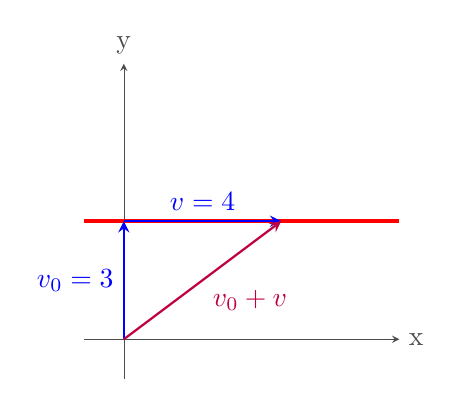
\begin{tikzpicture}[>=stealth]
	% les axes
	\draw[->,very thin,black!70] (-0.5,0) -- (3.5,0) node[anchor=west]{x};
	\draw[->,very thin,black!70] (0,-0.5) -- (0,3.5) node[anchor=south]{y};
	% la droite
	\draw[-, ultra thick, red] (-0.5,1.5 ) -- (3.5, 1.5);
	% les vecteurs
	\draw[->, thick,blue] (0, 0) -- node[anchor=east]{$\vect{v}_0 = 3\junit$} (0,1.5);
	\draw[->, thick,blue] (0, 1.5) -- node[anchor=south]{$\vect{v} = 4\iunit$} (2,1.5);
	\draw[->, thick,purple] (0, 0) -- node[anchor=north west]{$\vect{v}_0 + \vect{v}$} (2,1.5);
\end{tikzpicture}
\caption{\label{fig:droite1} La droite $y=3$, indiquée en rouge.}
\end{minipage}\hfill
\begin{minipage}{0.45\textwidth}

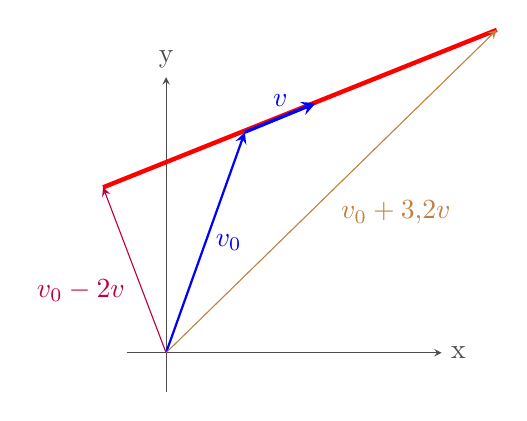
\begin{tikzpicture}[>=stealth]
    % les axes
	\draw[->,very thin,black!70] (-0.5,0) -- (3.5,0) node[anchor=west]{x};
	\draw[->,very thin,black!70] (0,-0.5) -- (0,3.5) node[anchor=south]{y};
	% la droite
	\draw[-, ultra thick, red] (-0.8,2.1 ) -- (4.2, 4.1);
	% les vecteurs
	\draw[->,very thick,blue] (1,2.8) -- node[anchor=south]{$\vect{v}$} (1.9,3.17);
	\draw[->,thick, blue] (0, 0) -- node[anchor= west]{$\vect{v}_0$} (1,2.8);
	\draw[->,brown] (0, 0) -- node[anchor=north west]{$\vect{v}_0 + 3{,}2\vect{v}$} (4.2,4.1);
	\draw[->,purple] (0, 0) -- node[anchor=north east]{$\vect{v}_0 - 2\vect{v}$} (-0.8,2.1);
\end{tikzpicture}
\caption{\label{fig:droite2} Une droite arbitraire dans le plan.}

\end{minipage}
\end{figure}


Est-ce que l'équation sous forme paramétrique est toujours valable dans l'espace à trois dimensions?  \\
Réponse: oui, contrairement à l'équation $y=mx+b$ qui, dans ce cas et comme nous le verrons,
représente un plan!  On peut obtenir l'équation
d'une droite en termes de coordonnées de la façon suivante.
\[
\begin{matrix}[rcl]
\vect{r} &=& \vect{v}_0 + t \vect{v} \\
\Rightarrow\quad (x, y, z) &=& (x_0, y_0, z_0) + t(v_1,v_2, v_3) \\
\Rightarrow && \left\{ \begin{matrix}
x-x_0 = tv_1 \\
y - y_0 = t v_2 \\
z-z_0 = t v_3
\end{matrix}\right.
\end{matrix}
\]
Puisque le paramètre $t$ est le même dans les trois équations, on écrit habituellement ceci
comme
\[
{\color{red}t =}\qquad \frac{x-x_0}{v_1} =\frac{y-y_0}{v_2} =\frac{z-z_0}{v_3}
\]
sans inclure le paramètre $t$ et où on suppose qu'aucuns des dénominateurs n'est égal
à zéro.  
En fait, habituellement, on ne connait pas le vecteur
directeur $\vect{v}$ mais on connait deux points; à partir de ces points, on
peut obtenir $\vect{v}$ de la façon suivante:
\[
\vect{v} = \overrightarrow{OP_1} - \overrightarrow{OP_0} = (x_1-x_0, y_1-y_0, z_1-z_0)
\]
de telle sorte que l'équation sous forme symétrique devient
\[
\frac{x-x_0}{x_1-x_0} =\frac{y-y_0}{y_1-y_0} =\frac{z-z_0}{z_1-z_0}
\]
et en se rappelant que si l'un des dénominateurs s'annule (par exemple $z_1=z_0$),
alors le numérateur doit s'annuler également (par exemple $z = z_0$).  Cette façon d'écrire
l'équation d'une droite est parfois appelée la \definition{forme symétrique}. Lorsqu'une droite
est exprimée ainsi, on voit que ça correspond bien
au fait qu'on ne peut avoir qu'une seule droite qui passe par deux points distincts;
les points ici seraient $P_0 =  (x_0, y_0, z_0)$ et $P_1 =  (x_1, y_1, z_1)$.

\begin{exemple}
Soit l'équation d'une droite \textbf{dans le plan} exprimée sous la forme traditionnelle:
\[
y = 2x + 3
\]
Obtenez une forme paramétrique de cette droite ainsi qu'une forme symétrique.
\solution
La façon la plus simple est de trouver deux points appartenant à cette droite.
Par exemple, si on choisis $x=1$ alors on aura $y=5$.  Appelons ce point $P_0 = (1,5)$.
On peut choisir un autre point, par exemple $P_1 = (2,7)$.  En utilisant ces valeurs,
on peut obtenir directement la forme symétrique comme suit:
\[
\frac{x-1}{2-1} = \frac{y-5}{7-5} \qquad \Rightarrow \qquad x-1 = \frac{y-5}{2}
\]
On peut vérifier facilement que cette équation est équivalente à l'équation dans sa forme traditionnelle.

Pour obtenir la forme paramétrique, on écrit 
\[
\vect{v} =\overrightarrow{P_1P_0} = \overrightarrow{OP_1} - \overrightarrow{OP_0} = (2,7) - (1,5) = (1,2)
\]
et donc
\[
\vect{r} = (x,y) = (1,5) + t (1,2)
\]
On peut vérifier que si $t=0$ alors $\vect{r} = P_0$, et si $t=1$, alors $\vect{r} = P_1$.
\end{exemple}

\section{Distance d'un point à une droite}

Soit une droite obéissant l'équation $\vect{r} = \vect{v}_0 + t \vect{v}$; on veut
trouver la distance entre cette droite et un point $P$.  Pour trouver cette distance,
on commence par choisir un point arbitraire de la droite.  Puisqu'on connait déjà
le point $P_0$ défini par $\overrightarrow{OP_0} = \vect{v}_0$, c'est le point qu'on
va utiliser, bien que tout autre point pourrait être choisi. Si $P=P_0$, il est évident
que la distance recherchée est zéro; dans ce qui suit, nous allons considérer le cas
$P\neq P_0$.
 En raison de la loi d'addition des vecteurs, nous avons
\[
\overrightarrow{OP_0} + \overrightarrow{P_0 P} = \overrightarrow{OP}
\]

\begin{figure}[h]
\begin{minipage}{0.45\textwidth}
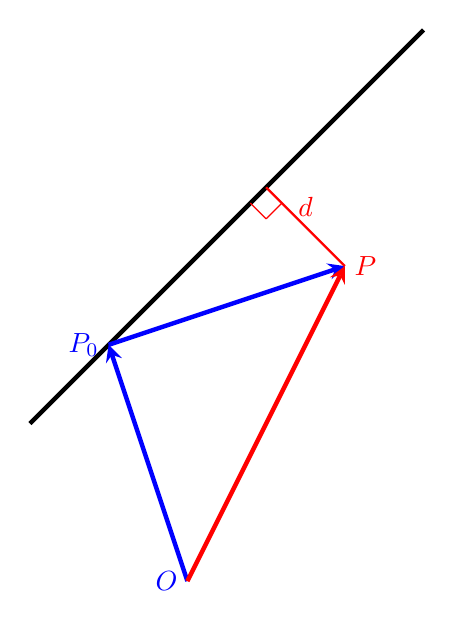
\begin{tikzpicture}[>=stealth]
	\coordinate [label=left:\textcolor{blue}{$P_0$}] (P0) at (-1,3);
	\coordinate [label=left:\textcolor{blue}{$O$}] (O) at (0,0);
	\coordinate [label=right:\textcolor{red}{$P$}] (P) at (2,4);
	\coordinate  (C) at (1,5);

	% la droite
	\draw[-, ultra thick, black] (-2,2 ) -- (3,7);
	\draw[->, ultra thick, blue] (O) -- (P0);
	\draw[->, ultra thick, blue] (P0) -- (P);
	\draw[->, ultra thick, red] (O) -- (P);
	\draw[-, thick, red] (C) -- node[anchor=south] {\textcolor{red}{$d$}} (P);
	\draw[-, thin, red] (0.8,4.8) -- (1,4.6);
	\draw[-, thin, red] (1,4.6) -- (1.2,4.8);

\end{tikzpicture}
\caption{\label{fig:DistDroitePoint1} Distance entre le point $P$ et la
droite passant par le point $P_0$.}
\end{minipage}\hfill
\begin{minipage}{0.45\textwidth}

\begin{tikzpicture}[>=stealth]

	\coordinate [label=left:\textcolor{blue}{$P_0$}] (P0) at (-1,3);
	\coordinate [label=right:\textcolor{blue}{$P$}] (P) at (2,4);
	\coordinate  (C) at (1,5);

	\draw[-, black] (-2,2 ) -- (3,7);
	\draw[->, very thick, blue] (P0) -- (P);
	\draw[-, very thick, blue] (C) -- node[anchor=south] {$d$}(P);
	% le vecteur v_0
	\draw[->,very thick,blue] (P0) -- node[anchor=south]{$\vect{v}$} node[anchor= west]{\textcolor{black}{$\theta$}} (0,4);
	\draw (0.2,3.4) arc (20:58:9mm);

\end{tikzpicture}
\caption{\label{fig:DistDroitePoint2} Visualisation de l'angle $\theta$ entre
le vecteur directeur $\vect{v}$ et le vecteur joignant les points $P_0$ et $P$.}

\end{minipage}
\end{figure}




Si on observe la figure \ref{fig:DistDroitePoint2} on observe que la distance 
recherchée est $d$ qui est
le côté opposé à l'angle $\theta$ du triangle rectangle dont l'hypoténuse est
égale à $\overrightarrow{P_0 P}$. Donc, nous avons
\[
d = \norm{\overrightarrow{P_0P}}\sin\theta
\]
Nous savons également que la norme du produit vectoriel $\vect{v} \times \overrightarrow{P_0 P}$
est
\[
\norm{\vect{v} \times \overrightarrow{P_0 P}} = v \norm{\overrightarrow{P_0 P}} \sin\theta
\]
En comparant ces deux expressions, on obtient
\[
d = \frac{\norm{\vect{v} \times \overrightarrow{P_0 P}}}{\norm{\overrightarrow{P_0 P}}}
\]
qui est le résultat recherché.


\begin{exemple}
Trouver l'équation paramétrique ainsi que l'équation sous forme symétrique de la droite
passant par les points $P_0 = (3, 4, 0)$ et $P_1 = (2, 4, 5)$.  De plus, trouver la distance entre
le point $P=(1, 2, 3)$ et cette droite.
\solution
Un vecteur directeur est donné par un multiple du vecteur $\overrightarrow{P_0P_1}$:
\[
\vect{v} = \overrightarrow{P_0P_1} = \overrightarrow{OP_1} - \overrightarrow{OP_0} = (2,4,5)-(3,4,0) = (-1,0,5) 
\]
Similairement, on peut choisir $\vect{v}_0 = \overrightarrow{OP_0} = (3,4,0)$ et donc l'équation
paramétrique peut être écrite comme
\[
\vect{r} = (3,4,0) + t(-1,0,5)
\]
La forme symétrique de la droite est obtenue directement à partir des points originaux \textbf{mais}
en notant que $y$ est constant:
\[
y=4 \quad\mbox{et}\quad \frac{x-3}{2-3} = \frac{z-0}{5-0} \qquad \Rightarrow\qquad  \frac{x-3}{-1} = \frac{z}{5}
\]
À noter que, si on avait interchangé $P_0$ et $P_1$ et tenter d'utiliser l'équation telle que nous l'avions
dérivée, nous aurions obtenu une division par zéro, ce qui n'est évidemment pas permis.  Donc, pour obtenir
une forme symétrique, on doit parfois obtenir en premier la forme paramétrique, en déduire la valeur de deux
points distincts qui n'ont pas de composantes de coordonnées qui sont nulles, et ensuite utiliser ces deux
points pour obtenir une forme symétrique.

La distance du point $P$ à cette droite est obtenue simplement en calculant
\[
d = \frac{\norm{\vect{v} \times \overrightarrow{P_0 P}}}{\norm{\overrightarrow{P_0 P}}}
\]
où $\overrightarrow{P_0 P} = (1,2,3)-(3,4,0)= (-2,-3,3)$et donc
\[
d = \frac{\norm{(-1,0,5)\times (-2,-2,3)}}{\norm{(-2,-3,3)}}
\]
Mais
\[
(-1,0,5)\times (-2,-2,3) = \begin{vmatrix}
\iunit & \junit & \kunit \\
-1 & 0 & 5 \\
-2 & -2& 3
\end{vmatrix}
=
\iunit\begin{vmatrix}
0 & 5 \\
-2 & 3
\end{vmatrix}
- \junit\begin{vmatrix}
-1 & 5 \\
-2 & 3
\end{vmatrix} + k\begin{vmatrix}
-1 & 0 \\
-2 & -2
\end{vmatrix}
=
10\iunit -7\junit + 2\kunit
\]
et donc
\[
d = \frac{\norm{(10,-7,2)}}{\norm{(-2,-2,3)}} = \frac{\sqrt{153}}{\sqrt{17}}
\]
\end{exemple}

\begin{exerciceC}
Trouver l'équation paramétrique ainsi que l'équation sous forme symétrique de la droite
passant par les points $P_0 = (9,0,3)$ et\\ $P_1 = (5,3,0)$.  De plus, trouver la distance entre
l'origine et cette droite.
\end{exerciceC}
\begin{exerciceC}
Trouver l'équation paramétrique ainsi que l'équation sous forme symétrique de la droite
passant par les points $P_0 = (1, 2, 3)$ et\\ $P_1 = (4, -1, 7)$.  De plus, trouver la distance entre
le point $P=(2,-5,1)$ et cette droite.
\end{exerciceC}


\section{Équation d'un plan}

Soit deux vecteurs linéairement indépendants\footnote{On dit de deux vecteurs linéairement \textbf{dépendants} qu'ils sont \textbf{colinéaires}.}, $\vect{v}_1$ et $\vect{v}_2$.  L'ensemble des points formés par l'ensemble de toutes
les combinaisons linéaires de ces deux vecteurs forme un plan passant par l'origine.  Si on ajoute à chacune
de ces combinaisons linéaires un vecteur constant $\vect{v}_0$, on peut obtenir n'importe quel plan $\Pi$
dans l'espace euclidien
\[
\Pi: \vect{r} = \vect{v}_0 + s\vect{v}_1 + t\vect{v}_2 
\]
Cette équation vectorielle est équivalente aux trois équations paramétriques suivantes:
\[
\left\{ \begin{matrix}[rcl]
x &=& x_0 + s\,x_1 + t\,x_2 \\
y &=& y_0 + s\,y_1 + t\,y_2 \\
z &=& z_0 + z\,x_1 + t\,z_2 
\end{matrix}\right.
\]

On peut démontrer qu'on peut trouver une expression équivalente appelée l'\definition{équation cartésienne du plan}
\[
Ax + By + Cz + D = 0
\]
Soit le point $P = (x, y, z)$ appartenant au plan $\Pi$; le vecteur $\overrightarrow{P_0P}$ sera donc 
dans le plan engendré par les vecteurs $\vect{v}_1$  et $\vect{v}_2$. Par la définition du produit
mixte, on sait que
\[
-\overrightarrow{P_0P} \cdot (\vect{v}_1 \times \vect{v}_2) = 0
\]
où on a choisit de mettre un signe - devant l'expression simplement pour
changer l'ordre des termes dans une expression à venir pour faciliter la comparaison
avec l'équation cartésienne du plan écrite ci-dessus.
Si on écrit $\overrightarrow{P_0P} = \overrightarrow{OP_0} - \overrightarrow{OP}$, le produit mixte ci-dessus
peut être écrit comme la différence de deux déterminants
\[
0 = \begin{vmatrix}
\overrightarrow{OP}\\
\vect{v}_1 \\
\vect{v}_2
\end{vmatrix} 
-
\begin{vmatrix}
\overrightarrow{OP_0}\\
\vect{v}_1 \\
\vect{v}_2
\end{vmatrix} 
\]
On peut récrire ceci comme
\[
0 = \begin{vmatrix}
x & y & z \\
x_1 & y_1 & z_1 \\
x_2 & y_2 & z_2
\end{vmatrix}
-
\begin{vmatrix}
x_0 & y_0 & z_0 \\
x_1 & y_1 & z_1 \\
x_2 & y_2 & z_2
\end{vmatrix}
\]
Faisons l'expansion de ces deux déterminants selon la première ligne.
\begin{align*}
0 =\quad & x \begin{vmatrix}
y_1 & z_1\\
y_2 & z_2
\end{vmatrix}
-
y \begin{vmatrix}
x_1 & z_1 \\
x_2 & z_2
\end{vmatrix}
+
z \begin{vmatrix}
x_1 & y_1 \\
x_2 & y_2
\end{vmatrix} \\
& -x_0 \begin{vmatrix}
y_1 & z_1\\
y_2 & z_2
\end{vmatrix}
+
y_0 \begin{vmatrix}
x_1 & z_1 \\
x_2 & z_2
\end{vmatrix}
-
z_0 \begin{vmatrix}
x_1 & y_1 \\
x_2 & y_2
\end{vmatrix}
\end{align*}
Définissons les trois variables suivantes:
\[
\begin{matrix}[rcl]
A &=& \begin{vmatrix}
y_1 & z_1\\
y_2 & z_2
\end{vmatrix}\\
B &=& - \begin{vmatrix}
x_1 & z_1 \\
x_2 & z_2
\end{vmatrix} \\
C&=& \begin{vmatrix}
x_1 & y_1 \\
x_2 & y_2
\end{vmatrix}
\end{matrix}
\]
Ceci nous permet d'obtenir l'expression recherchée
\[
Ax + By + Cz - (Ax_0 + By_0 + Cz_0) = Ax + By + Cz + D = 0
\]
où $D = - (Ax_0 + By_0 + Cz_0)$.

De plus, on observe que $\vect{v}_1 \times \vect{v}_2 = (A, B, C)$ est un vecteur
orthogonal au plan.  Au lieu du mot orthogonal, on utilise
habituellement le mot \definition{normal}{}\footnote{Perpendiculaire, 
orthogonal et normal sont presque des synonymes.  Ceci peut parfois porter à confusion,
d'autant plus si l'on inclut un faux ami comme la norme (ou longueur) d'un vecteur ainsi
que l'adjectif normé, signifiant de longueur unitaire. [normé $\neq$ normal]  On a vu une combinaison de 
deux termes avec les bases orthonormées qui décrivent des vecteur orthogonaux (le préfixe ortho) 
de longueur unitaire (le suffixe normées).  Cela dit, on utilise habituellement l'adjectif
orthogonal lorsqu'on veut décrire la propriété de deux objets semblables (par exemple: des
vecteurs orthogonaux) et l'adjectif normal lorsque les deux objets sont différents (par exemple:
le vecteur normal à un plan ou à une droite).  L'adjectif perpendiculaire est réservé aux 
objets qui se trouvent dans un même plan.}.

Finalement, on note que si on a $C=0$, on peut définir $m = -A/B$ et $b= -D/A$ ce qui nous
permet d'avoir l'équation du plan $y=mx+b$ !

\section{Distance d'un point à un plan}

Soit un point\footnote{Nous avons choisi d'utiliser les variables $x, y, z$ pour
dénoter les coordonnées du point. Par contre, tel qu'il est indiqué dans le texte, ceci ne veut
\textbf{pas} nécessairement dire que ces coordonnées obéiront l'équation $Ax+By+Cz+D=0$.}
 $P=(x, y, z)$.  
On veut trouver la distance de ce point au plan donné par l'équation cartésienne
\[
\Pi: Ax + By + Cz + D = 0
\]

\begin{figure}[h]
\begin{tikzpicture}
	\coordinate [label=left:\textcolor{blue}{$\Pi$}] (A0) at (0, 0);
	\coordinate (B0) at (3, 3);
	\coordinate (C0) at (9, 0);
	\coordinate (D0) at (11.5, 3);
	\coordinate [label=right:{$P = (x,y,z)$}] (P) at (6, 5);
	\coordinate [label=below:{$\quad P_\perp$}] (Pp) at (6, 1.5);
	\coordinate [label=left:{$P_1$}] (P1) at (5.2, 2.1);
	\coordinate [label=right:{$P_2$}] (P2) at (7,2);
% initial area
\begin{pgfonlayer}{background}
   \path [fill=blue!10] (A0) -- (B0) -- (D0) -- (C0) -- (A0);
\end{pgfonlayer}
	\draw[-,thick,black] (Pp) -- (P);
	\draw[->,ultra thick,red] (Pp) -- node[anchor=east]{\textcolor{red}{$\vect{n}$}} (6,3) ;
	\filldraw (P) circle (0.7mm);
	\filldraw (Pp) circle (0.7mm);
	\draw[dashed] (Pp) -- (P1);
	\draw[dashed] (Pp) -- (P2);
	\draw[dashed] (P) -- (P1);
	\draw[dashed] (P) -- (P2);
	\draw[densely dotted] (5.8,1.7) -- (5.8,1.85);
	\draw[densely dotted] (5.8,1.85) -- (6,1.7);
	\draw[densely dotted] (6.2,1.62) -- (6.2,1.8);
	\draw[densely dotted] (6.2,1.8) -- (6,1.68);
\end{tikzpicture}

\caption{\label{fig:DistPointPlan}
La distance du point $P$ au plan $\Pi$ égale à la longueur du segment de droite
joignant les points $P$ et $P_\perp$; cette distance est inférieure à la distance entre
$P$ et tout autre point du plan, tel que $P_1$ ou $P_2$.
Notez que le point aurait pu être choisi sous le plan, et donc dans une direction
opposée à celle du vecteur normal indiqué sur la figure.
}
\end{figure}






Cette distance sera égale à la longueur du segment de droite joignant le point $P$ à
sa projection sur le plan indiquée par le point $P_\perp$.
Pour fins de clarification, il est important de noter que le point   $P_\perp$ appartient
au plan $\Pi$ et que nous avons donc
\[
\Pi: Ax_\perp + By_\perp + Cz_\perp + D = 0
\]
Par contre, le point $P$ n'appartient pas nécessairement au plan $\Pi$.

Le segment de droite joignant les points $P_\perp$ et $P$ est colinéaire à la normale
de ce plan que nous désignons par $\vect{n}$.  Nous avons donc $\overrightarrow{P_\perp P} = k \vect{n}$, et
la distance recherchée est donc
\[
d = \norm{\overrightarrow{P_\perp P}} = |k|\, \norm{\vect{n}}
\]
Nous avons vu précédemment que le vecteur $(A, B, C)$ était un vecteur normal au plan.
Ceci nous permet d'écrire
\[
\begin{pmatrix}
x_\perp-x, 
 y_\perp-y, 
 z_\perp-z
\end{pmatrix}
= k \begin{pmatrix}
A, B , C
\end{pmatrix}
\]
Nous avons donc le système d'équations linéaires suivant:
\[
\left\{
\begin{matrix}[rcl]
x_\perp &=& x + kA \\
y_\perp &=& y + kB \\
z_\perp &=& z + kC \\
Ax_\perp + By_\perp + Cz_\perp + D &=& 0
\end{matrix}
\right.
\]
En substituant les valeurs des variables des trois premières équations dans la quatrième, on trouve
\[
Ax + By + Cz + D + k( A^2 + B^2 + C^2 ) = 0
\]
Pour un plan quelconque, il peut arriver que l'une, voire deux des
variables $A, B, C$ soit égale à zéro, mais jamais les trois
en même temps. Donc, nous avons
\[
k = -\frac{Ax + By + Cz + D}{A^2 + B^2 + C^2}
\]
ce qui nous permet d'écrire
\[
d =  |k|\, \norm{\vect{n}} = \frac{|Ax + By + Cz + D|}{A^2 + B^2 + C^2} \sqrt{A^2 + B^2 + C^2}
\]
et donc
\[
d = \frac{|Ax + By + Cz + D|}{\sqrt{A^2 + B^2 + C^2}} 
\]
On observe que si le point $P$ appartient au plan, alors le numérateur s'annule et la distance
au plan est évidemment égale à zéro. 

\begin{exemple}
Obtenez l'équation cartésienne du plan passant par les points $P_1=(1,0,0)$, $P_2=(0,1,0)$ et $P_3=(0,0,1)$ et
déterminez la distance entre l'origine et ce plan.
\solution
Avant de présenter la solution, nous notons qu'aucun des points n'est indiqué comme étant le point $P_0$. Ceci n'est
pas un hasard: bien que dans la dérivation, le point $P_0$ semble jouer un rôle particulier, dans la pratique on
peut choisir n'importe quel point comme étant le point $P_0$ de la dérivation.  Nous commençons par choisir
deux vecteurs qui sont parallèles au plan:
\[
\vect{v}_1 = \overrightarrow{P_2P_3} = (0,0,1) - (0,1,0) = (0,-1,1)
\]
et 
\[
\vect{v}_1 = \overrightarrow{P_1P_3} = (0,0,1) - (1,0,0) = (-1,0,1)
\]
Choisissons ensuite le point $P_3$ pour jouer le rôle du point $P_0$ de notre dérivation.  Nous devons avoir
\[
0 = -\overrightarrow{P_3P} \cdot (\vect{v}_1 \times \vect{v}_2) = \begin{vmatrix}
\overrightarrow{OP}\\
\vect{v}_1 \\
\vect{v}_2
\end{vmatrix} 
-
\begin{vmatrix}
\overrightarrow{OP_3}\\
\vect{v}_1 \\
\vect{v}_2
\end{vmatrix} =\begin{vmatrix}
x & y & z \\
0 & -1 & 1 \\
-1 & 0 & 1
\end{vmatrix}
-
\begin{vmatrix}
0 & 0 & 1 \\
0 & -1 & 1 \\
-1 & 0 & 1
\end{vmatrix} = -x-y-z+1
\]
et donc l'équation cartésienne du plan peut s'écrire: $x+y+z=1$.  On peut
vérifier facilement que les trois points qui nous étaient donnés satisfont cette équation.
Si on compare avec la forme $Ax+By+Cz+D=0$, on a $A=B=C=1$ et $D=-1$.

La distance d'un point à un plan est donnée par l'équation 
\[
d = \frac{|Ax + By + Cz + D|}{\sqrt{A^2 + B^2 + C^2}} 
\]
Ici, le point qui nous intéresse est l'origine $(0,0,0)$ et donc la distance recherchée est
\[
d = \frac{1}{\sqrt{1^2 + 1^2 + 1^2}} = \frac{1}{\sqrt{3}} = \frac{\sqrt{3}}{3}
\]
\end{exemple}

\begin{exerciceC}
Obtenez l'équation cartésienne du plan passant par les points $P_1=(1,2,3)$, $P_2=(1,-3,2)$ et $P_3=(0,0,1)$ et
déterminez la distance entre le point $P=(2,2,2)$ et ce plan.
\end{exerciceC}
\begin{exerciceC}
Obtenez l'équation cartésienne du plan passant par les points $P_1=(4,-3,6)$, $P_2=(5,2,-8)$ et $P_3=(3,1,2)$ et
déterminez la distance entre le point $P=(1,2,3)$ et ce plan.
\end{exerciceC}